\section{Context}

\paragraph{}
The synthesis of insights from the \gls{ipcc}'s 2023 report[\cite{IPCC_SynthesisReport2023}] and the \gls{un}' "The \gls{sdg} Report 2023"[\cite{UN_SDGReport2023}] offers a comprehensive view on the multifaceted approach required to address climate change. These documents underscore the importance of sustainability, \gls{energyEfficiency}, and \gls{energyResilience} within the realms of \gls{iot} and \gls{eh}. Together, they pave the way toward a sustainable, efficient, and resilient energy future, highlighting the interplay between these factors in global efforts to mitigate climate change impacts.

\subsection{Overview}

    \paragraph{}
    The \gls{ipcc}'s 2023 report[\cite{IPCC_SynthesisReport2023}], alongside the \gls{un}'s 2023 \gls{sdg} report[\cite{UN_SDGReport2023}], underscores the urgent need for comprehensive strategies to combat the far-reaching effects of climate change. These reports emphasize the importance of sustainable development pathways, integrating inclusive governance, diverse knowledge, and innovative solutions to ensure resilient societies and ecosystems.


\subsection{Sustainability}

    \paragraph{}
    Sustainability, as detailed within \gls{eh} and \gls{iot} applications and outlined by the UN's sustainability goals, involves a balanced approach to environmental integrity, social equity, and economic viability[Fig 1: The Sustainability Triangle\ref{fig:sustainabilityTriangle}]. These technologies offer opportunities to reduce environmental impacts, enhance social inclusion, and foster economic growth through innovative solutions that minimize resource use and improve energy access.
    \begin{itemize}
        \item \textbf{Environmental} Aspect: Emphasizes renewable energy sources and energy-efficient designs to reduce carbon footprints and environmental degradation.
        \item \textbf{Social} Aspect: Focuses on enhancing accessibility, safety, and community well-being through equitable energy solutions and stakeholder engagement.
        \item \textbf{Economic} Aspect: Highlights cost savings and economic growth potential through innovative energy solutions and market creation.
    \end{itemize}
    
    \begin{figure}[htbp]
        \centering
        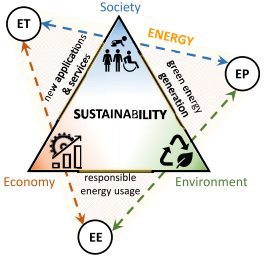
\includegraphics[width=0.5\textwidth]{img/005_SustainabilityTriangle.png}
        \caption{The Sustainability Triangle, highlighting the critical balance between environmental, social, and economic factors in achieving sustainable outcomes\cite{EnergySustainableIoT}.}
        \label{fig:sustainabilityTriangle}
    \end{figure}

\newpage
\subsection{Energy Efficiency}

    \paragraph{}
    \gls{energyEfficiency} is pivotal in reducing energy consumption and emissions. \gls{iot} devices enhance energy management across various sectors by enabling smart controls and predictive maintenance, while \gls{eh} technologies provide a sustainable energy supply by converting ambient energy into usable power.
    \begin{itemize}
        \item \textbf{\gls{iot}}: Enhances real-time energy monitoring and management, leading to significant energy savings and reduced waste\cite{HAFEZ2023101013}.
        \item \textbf{\gls{eh}}: Offers a renewable energy source, reducing reliance on traditional energy systems and enhancing device longevity\cite{LIU2023113436}.
    \end{itemize}

\subsection{Energy Resilience}

    \paragraph{}
    In the face of climate-induced disruptions, \gls{energyResilience} is increasingly critical. It involves the capacity of energy systems to withstand, adapt to, and recover from disturbances, ensuring stable and reliable energy supply\cite{iotSustainableEnergySystems}.
    \begin{itemize}
        \item \textbf{\gls{iot} for Resilience}: Employs real-time data and predictive analytics to enhance system responsiveness and recovery, contributing to a more distributed and less vulnerable energy infrastructure\cite{gameboyBatteryless}.
        \item \textbf{Energy Harvesting for Resilience}: Diversifies energy sources and enables autonomous operation, particularly beneficial in remote or disaster-prone areas, thus strengthening system robustness\cite{memsEHforIot}.
    \end{itemize}

\paragraph{}
The interconnectedness of \gls{sustainability}, \gls{energyEfficiency}, and \gls{energyResilience}, underpinned by \gls{iot}, \gls{mems} and \gls{eh} technologies, forms a cornerstone in the global response to climate change. Embracing these innovative approaches, as highlighted by the \gls{ipcc} and the UN's SDG reports, charts a path towards a sustainable, efficient, and resilient energy landscape. The collective pursuit of these objectives, in line with the urgent and inclusive climate action called for by these reports, is essential in mitigating climate impacts and securing a livable future for all.

Following the outlined context, we will delve into specific applications and the corresponding energy sources in the subsequent section.

\newpage
\subsection{Applications}

    \paragraph{}
    Below, we detail primary energy sources and their applications, as highlighted in \cite{greenIT} on page 8:
    \begin{itemize}
        \item \textbf{Motion} (\cite{eh_TorsionallyOscillatingMagnet}): This method encompasses \gls{electrostatic}, \gls{piezoelectric}, \gls{electromagnetic}, and \gls{magnetorestrictive} processes for powering IoT devices through movement. Its applications range from industrial uses, such as power transformers, to consumer technologies like battery-less gaming devices\cite{gameboyBatteryless}, vibration sensor in nuclear reactor\cite{iotSustainableEnergySystems}, to monitor and avert environmental radiation discharge.
        \item \textbf{Solar}: Utilizing light, \gls{photovoltaic} cells—both indoor and outdoor capable—serve as a versatile, renewable energy source crucial for infrastructure dependent on lighting schedules.
        \item \textbf{Thermal}: Exploiting temperature differentials allows for electricity generation useful in aerospace, automotive sensor enhancement, and wireless temperature management in food and pipelines, and for safety applications\cite{iotSustainableEnergySystems}.
        \item \textbf{Magnetic Field of Electric Power Lines}: Enhances electrical efficiency and transmission by harnessing naturally occurring magnetic fields.
        \item \textbf{Radio Frequency}: Key to \gls{rfid} technology, offering a sustainable alternative to standby modes in devices, conserving energy, and enabling early defect detection in maintenance.
        \item \textbf{Wind}: Facilitates environmental control in buildings through airflow energy harvesting.
    \end{itemize}

    \paragraph{}
    Additionally, beyond the succinct explanations provided for each energy source, numerous sectors will benefit significantly:
    \begin{itemize}
        \item \textbf{Healthcare}: Biometric wearables, harnessing motion energy, facilitate continuous health monitoring without battery dependence.
        \item \textbf{Maintenance Operations}: Energy sources across various sectors predict maintenance needs, adapt operations, and optimize consumption.
        \item \textbf{Military Operations}: \gls{terraswam} including \gls{smartdust}.
    \end{itemize}
    
    \paragraph{}
    These innovations not only enhance \gls{ee} but also contribute significantly toward our sustainability goals.
    

    \begin{figure}[htbp]
        \centering
        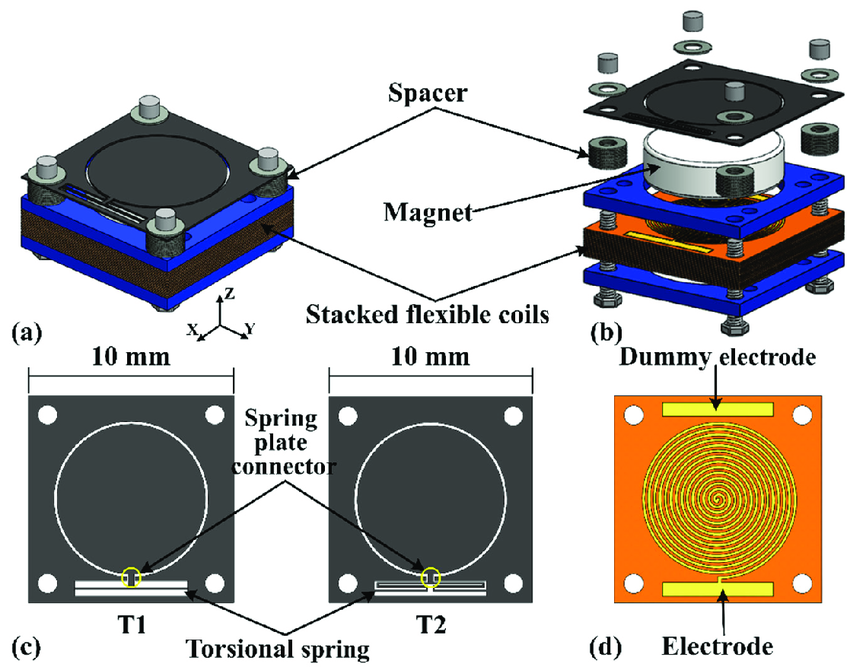
\includegraphics[width=0.5\textwidth]{img/006_EVEH.png}
        \caption{Schematic and exploded illustration of the assembled EVEH. (a) schematic illustration the \gls{eveh} device; (b) exploded view of the \gls{eveh} device; (c) two types of torsional spring; (d) layer of flexible coils\cite{eh_TorsionallyOscillatingMagnet}.}
        \label{fig:eveh}
    \end{figure}